\section{Résultats de la méthode}

\subsection{Résultats de la méthode}
    \begin{frame}
        \frametitle{Résultats de la méthode}
        Intégration des classificateurs développés précédemment :
        \begin{enumerate}
            \item classificateur proprioceptif basé sur les vibrations et classificateur extéroceptif ;
            \item classificateur basé sur le coefficient de traction et classificateur extéroceptif.
        \end{enumerate}         
    \end{frame}

\subsection{Résultats pour l'approche par vibration}
    \begin{frame}
        \frametitle{Approche par vibrations}
        Évaluation du rapport entre les VP et les FP.
        \begin{center}              
            \begin{tabular}{|lcc|}
                \hline
                Classe & VP (\%) &  FP (\%)\\
                \hline
                Roche & > 25 & < 1,5 \\
                Herbes & > 80 & < 1 \\
                Sable & > 80 & < 1\\
                \hline           
            \end{tabular}                  
        \end{center} 
        Les résultats de l'apprentissage auto-supervisé sont presque aussi bon que ceux supervisés manuellement. 
    \end{frame}

\subsection{Résultats pour l'approche par coefficient de traction}
    \begin{frame}
        \frametitle{Approche par coefficient de traction}
        \begin{itemize}
            \item Classement attribué selon le coefficient de traction (A,B,C,D,E).
            \item Estimation conservatrice de $\mu_{tr}$ : P($\mu_{tr}>$ valeur réelle) $\geq$ 80\%.            
            \begin{itemize}
                 \item évaluation par une somme pondérée des bornes inférieur des classes selon la probabilité d'appartenance à la classe.
                 \item Malheureusement, aucune valeur de référence n'était disponible.
            \end{itemize}
        \end{itemize}
    \end{frame}
    
    \begin{frame}[c]
        \begin{center}
            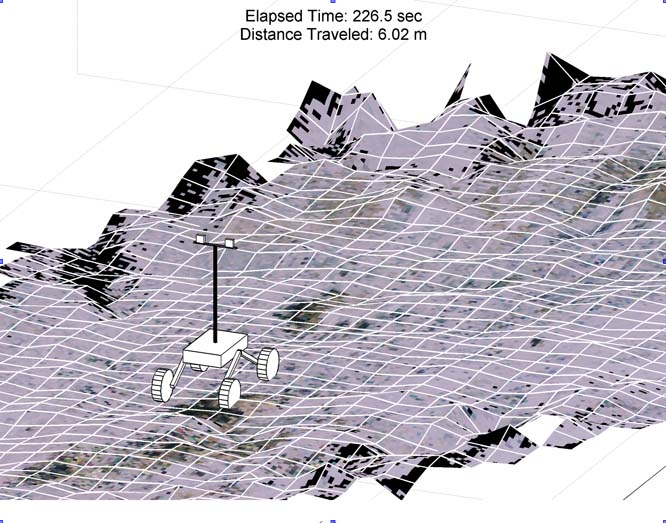
\includegraphics[height=0.8\textheight]{./media/resultatCarte.jpg}
        \end{center}        
    \end{frame}
    
    \begin{frame}[c]
        \begin{center}
            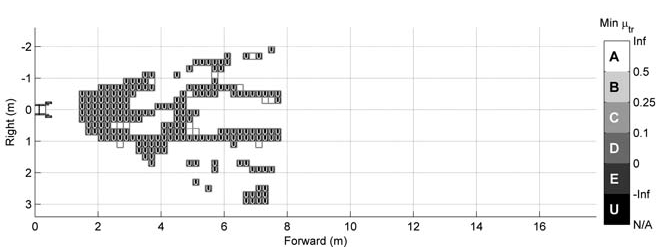
\includegraphics[width=\textwidth]{./media/resultat1.jpg}
        \end{center}        
    \end{frame}
    
    \begin{frame}[c]
        \begin{center}
            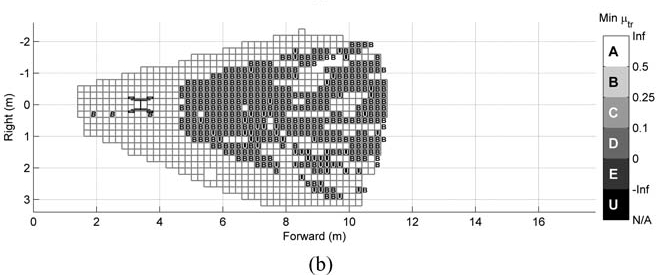
\includegraphics[width=\textwidth]{./media/resultat2.jpg}
        \end{center}        
    \end{frame}
    
    \begin{frame}[c]
        \begin{center}
            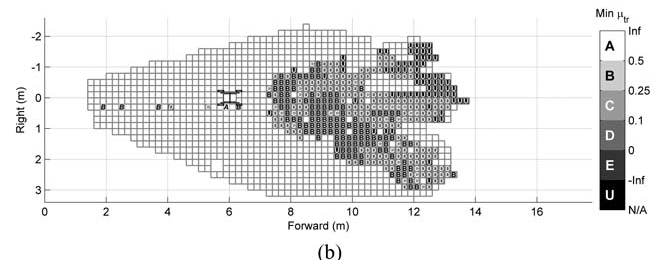
\includegraphics[width=\textwidth]{./media/resultat3.jpg}
        \end{center}        
    \end{frame}    
    
\subsection{Conclusion}
    \begin{frame}
        \frametitle{Conclusion}
        \begin{itemize}
            \item Approche de classification auto-supervisé pour la prédiction distante des contraintes non géométriques du terrains.
            \item Deux approche de classement proprioceptif:
            \begin{itemize}
                \item vibrations, coefficient de traction.
            \end{itemize}
            \item Un classement extéroceptif basé sur trois types d'information.
            \begin{itemize}
                \item couleurs, textures visuelles et géométrie du terrain.
            \end{itemize}
            \item Résultats prometteurs grâce aux expérimentations (TORTOISE ,Wingaersheek).
        \end{itemize}
    \end{frame}
